\documentclass[twoside]{book}

% Packages required by doxygen
\usepackage{fixltx2e}
\usepackage{calc}
\usepackage{doxygen}
\usepackage[export]{adjustbox} % also loads graphicx
\usepackage{graphicx}
\usepackage[utf8]{inputenc}
\usepackage{makeidx}
\usepackage{multicol}
\usepackage{multirow}
\PassOptionsToPackage{warn}{textcomp}
\usepackage{textcomp}
\usepackage[nointegrals]{wasysym}
\usepackage[table]{xcolor}

% Font selection
\usepackage[T1]{fontenc}
\usepackage[scaled=.90]{helvet}
\usepackage{courier}
\usepackage{amssymb}
\usepackage{sectsty}
\renewcommand{\familydefault}{\sfdefault}
\allsectionsfont{%
  \fontseries{bc}\selectfont%
  \color{darkgray}%
}
\renewcommand{\DoxyLabelFont}{%
  \fontseries{bc}\selectfont%
  \color{darkgray}%
}
\newcommand{\+}{\discretionary{\mbox{\scriptsize$\hookleftarrow$}}{}{}}

% Page & text layout
\usepackage{geometry}
\geometry{%
  letterpaper,%
  top=2.5cm,%
  bottom=2.5cm,%
  left=2.5cm,%
  right=2.5cm%
}
\tolerance=750
\hfuzz=15pt
\hbadness=750
\setlength{\emergencystretch}{15pt}
\setlength{\parindent}{0cm}
\setlength{\parskip}{3ex plus 2ex minus 2ex}
\makeatletter
\renewcommand{\paragraph}{%
  \@startsection{paragraph}{4}{0ex}{-1.0ex}{1.0ex}{%
    \normalfont\normalsize\bfseries\SS@parafont%
  }%
}
\renewcommand{\subparagraph}{%
  \@startsection{subparagraph}{5}{0ex}{-1.0ex}{1.0ex}{%
    \normalfont\normalsize\bfseries\SS@subparafont%
  }%
}
\makeatother

% Headers & footers
\usepackage{fancyhdr}
\pagestyle{fancyplain}
\fancyhead[LE]{\fancyplain{}{\bfseries\thepage}}
\fancyhead[CE]{\fancyplain{}{}}
\fancyhead[RE]{\fancyplain{}{\bfseries\leftmark}}
\fancyhead[LO]{\fancyplain{}{\bfseries\rightmark}}
\fancyhead[CO]{\fancyplain{}{}}
\fancyhead[RO]{\fancyplain{}{\bfseries\thepage}}
\fancyfoot[LE]{\fancyplain{}{}}
\fancyfoot[CE]{\fancyplain{}{}}
\fancyfoot[RE]{\fancyplain{}{\bfseries\scriptsize Generated by Doxygen }}
\fancyfoot[LO]{\fancyplain{}{\bfseries\scriptsize Generated by Doxygen }}
\fancyfoot[CO]{\fancyplain{}{}}
\fancyfoot[RO]{\fancyplain{}{}}
\renewcommand{\footrulewidth}{0.4pt}
\renewcommand{\chaptermark}[1]{%
  \markboth{#1}{}%
}
\renewcommand{\sectionmark}[1]{%
  \markright{\thesection\ #1}%
}

% Indices & bibliography
\usepackage{natbib}
\usepackage[titles]{tocloft}
\setcounter{tocdepth}{3}
\setcounter{secnumdepth}{5}
\makeindex

% Hyperlinks (required, but should be loaded last)
\usepackage{ifpdf}
\ifpdf
  \usepackage[pdftex,pagebackref=true]{hyperref}
\else
  \usepackage[ps2pdf,pagebackref=true]{hyperref}
\fi
\hypersetup{%
  colorlinks=true,%
  linkcolor=blue,%
  citecolor=blue,%
  unicode%
}

% Custom commands
\newcommand{\clearemptydoublepage}{%
  \newpage{\pagestyle{empty}\cleardoublepage}%
}

\usepackage{caption}
\captionsetup{labelsep=space,justification=centering,font={bf},singlelinecheck=off,skip=4pt,position=top}

%===== C O N T E N T S =====

\begin{document}

% Titlepage & ToC
\hypersetup{pageanchor=false,
             bookmarksnumbered=true,
             pdfencoding=unicode
            }
\pagenumbering{roman}
\begin{titlepage}
\vspace*{7cm}
\begin{center}%
{\Large Balance \\[1ex]\large 1.\+0 }\\
\vspace*{1cm}
{\large Generated by Doxygen 1.8.11}\\
\end{center}
\end{titlepage}
\clearemptydoublepage
\tableofcontents
\clearemptydoublepage
\pagenumbering{arabic}
\hypersetup{pageanchor=true}

%--- Begin generated contents ---
\chapter{Hierarchical Index}
\section{Class Hierarchy}
This inheritance list is sorted roughly, but not completely, alphabetically\-:\begin{DoxyCompactList}
\item \contentsline{section}{config\-\_\-file}{\pageref{classconfig__file}}{}
\item \contentsline{section}{logger\-\_\-col\-\_\-cfg}{\pageref{classlogger__col__cfg}}{}
\item \contentsline{section}{logger\-\_\-config}{\pageref{classlogger__config}}{}
\item \contentsline{section}{polydaq2}{\pageref{classpolydaq2}}{}
\item Task\-Base\begin{DoxyCompactList}
\item \contentsline{section}{task\-\_\-data\-\_\-acq}{\pageref{classtask__data__acq}}{}
\item \contentsline{section}{task\-\_\-leds}{\pageref{classtask__leds}}{}
\item \contentsline{section}{task\-\_\-pc}{\pageref{classtask__pc}}{}
\item \contentsline{section}{task\-\_\-print}{\pageref{classtask__print}}{}
\item \contentsline{section}{task\-\_\-sd\-\_\-card}{\pageref{classtask__sd__card}}{}
\item \contentsline{section}{task\-\_\-sd\-\_\-daq}{\pageref{classtask__sd__daq}}{}
\item \contentsline{section}{task\-\_\-user}{\pageref{classtask__user}}{}
\end{DoxyCompactList}
\end{DoxyCompactList}

\chapter{Class Index}
\section{Class List}
Here are the classes, structs, unions and interfaces with brief descriptions\-:\begin{DoxyCompactList}
\item\contentsline{section}{\hyperlink{classconfig__file}{config\-\_\-file} \\*Base class for a configuration file reader and parser }{\pageref{classconfig__file}}{}
\item\contentsline{section}{\hyperlink{classlogger__col__cfg}{logger\-\_\-col\-\_\-cfg} \\*Data for one sensor line in the logger configuration file }{\pageref{classlogger__col__cfg}}{}
\item\contentsline{section}{\hyperlink{classlogger__config}{logger\-\_\-config} \\*Parser for simple data logger configuration files }{\pageref{classlogger__config}}{}
\item\contentsline{section}{\hyperlink{classpolydaq2}{polydaq2} \\*Class which interacts with Poly\-D\-A\-Q 2 hardware }{\pageref{classpolydaq2}}{}
\item\contentsline{section}{\hyperlink{classtask__data__acq}{task\-\_\-data\-\_\-acq} \\*Task which acquires Poly\-D\-A\-Q data at precise time intervals }{\pageref{classtask__data__acq}}{}
\item\contentsline{section}{\hyperlink{classtask__leds}{task\-\_\-leds} \\*Task which pulses an L\-E\-D on and off as another responds to a button }{\pageref{classtask__leds}}{}
\item\contentsline{section}{\hyperlink{classtask__pc}{task\-\_\-pc} \\*Task for communication with the user or a P\-C based user interface }{\pageref{classtask__pc}}{}
\item\contentsline{section}{\hyperlink{classtask__print}{task\-\_\-print} \\*Task which prints out characters in the main print queue }{\pageref{classtask__print}}{}
\item\contentsline{section}{\hyperlink{classtask__sd__card}{task\-\_\-sd\-\_\-card} \\*Task which saves data to an S\-D card }{\pageref{classtask__sd__card}}{}
\item\contentsline{section}{\hyperlink{classtask__sd__daq}{task\-\_\-sd\-\_\-daq} \\*Task which acquires Poly\-D\-A\-Q data for the S\-D card }{\pageref{classtask__sd__daq}}{}
\item\contentsline{section}{\hyperlink{classtask__user}{task\-\_\-user} \\*Task for communication with the user or a P\-C based user interface }{\pageref{classtask__user}}{}
\end{DoxyCompactList}

\chapter{File Index}
\section{File List}
Here is a list of all documented files with brief descriptions\-:\begin{DoxyCompactList}
\item\contentsline{section}{\hyperlink{appconfig_8h}{appconfig.\-h} }{\pageref{appconfig_8h}}{}
\item\contentsline{section}{\hyperlink{config__file_8cpp}{config\-\_\-file.\-cpp} \\*Source code for a base class for small program configuration files }{\pageref{config__file_8cpp}}{}
\item\contentsline{section}{\hyperlink{config__file_8h}{config\-\_\-file.\-h} \\*Header for a base class for small program configuration files }{\pageref{config__file_8h}}{}
\item\contentsline{section}{\hyperlink{FreeRTOSConfig_8h}{Free\-R\-T\-O\-S\-Config.\-h} \\*Configuration settings for Free\-R\-T\-O\-S as it's used in this project }{\pageref{FreeRTOSConfig_8h}}{}
\item\contentsline{section}{\hyperlink{logger__config_8cpp}{logger\-\_\-config.\-cpp} \\*Source code for a parser for data logging configuration files }{\pageref{logger__config_8cpp}}{}
\item\contentsline{section}{\hyperlink{logger__config_8h}{logger\-\_\-config.\-h} \\*Headers for a parser for data logging configuration files }{\pageref{logger__config_8h}}{}
\item\contentsline{section}{\hyperlink{main_8cpp}{main.\-cpp} \\*The main file for the Poly\-D\-A\-Q 2 firmware }{\pageref{main_8cpp}}{}
\item\contentsline{section}{\hyperlink{polydaq2_8cpp}{polydaq2.\-cpp} }{\pageref{polydaq2_8cpp}}{}
\item\contentsline{section}{\hyperlink{polydaq2_8h}{polydaq2.\-h} \\*Headers for a class that drives the Poly\-D\-A\-Q 2 board's hardware }{\pageref{polydaq2_8h}}{}
\item\contentsline{section}{\hyperlink{shares_8h}{shares.\-h} \\*Declarations for inter-\/task data communication items (shares and queues) }{\pageref{shares_8h}}{}
\item\contentsline{section}{\hyperlink{task__data__acq_8cpp}{task\-\_\-data\-\_\-acq.\-cpp} }{\pageref{task__data__acq_8cpp}}{}
\item\contentsline{section}{\hyperlink{task__data__acq_8h}{task\-\_\-data\-\_\-acq.\-h} }{\pageref{task__data__acq_8h}}{}
\item\contentsline{section}{\hyperlink{task__leds_8cpp}{task\-\_\-leds.\-cpp} }{\pageref{task__leds_8cpp}}{}
\item\contentsline{section}{\hyperlink{task__leds_8h}{task\-\_\-leds.\-h} }{\pageref{task__leds_8h}}{}
\item\contentsline{section}{\hyperlink{task__pc_8cpp}{task\-\_\-pc.\-cpp} }{\pageref{task__pc_8cpp}}{}
\item\contentsline{section}{\hyperlink{task__pc_8h}{task\-\_\-pc.\-h} }{\pageref{task__pc_8h}}{}
\item\contentsline{section}{\hyperlink{task__sd__card_8cpp}{task\-\_\-sd\-\_\-card.\-cpp} \\*Source code for a task which saves data to an S\-D card }{\pageref{task__sd__card_8cpp}}{}
\item\contentsline{section}{\hyperlink{task__sd__card_8h}{task\-\_\-sd\-\_\-card.\-h} \\*Headers for a task which saves data to an S\-D card }{\pageref{task__sd__card_8h}}{}
\item\contentsline{section}{\hyperlink{task__sd__daq_8cpp}{task\-\_\-sd\-\_\-daq.\-cpp} }{\pageref{task__sd__daq_8cpp}}{}
\item\contentsline{section}{\hyperlink{task__sd__daq_8h}{task\-\_\-sd\-\_\-daq.\-h} }{\pageref{task__sd__daq_8h}}{}
\item\contentsline{section}{\hyperlink{task__user_8cpp}{task\-\_\-user.\-cpp} }{\pageref{task__user_8cpp}}{}
\item\contentsline{section}{\hyperlink{task__user_8h}{task\-\_\-user.\-h} }{\pageref{task__user_8h}}{}
\end{DoxyCompactList}

\chapter{Class Documentation}
\hypertarget{structaccelBuf}{}\section{accel\+Buf Struct Reference}
\label{structaccelBuf}\index{accel\+Buf@{accel\+Buf}}


Structure to hold 5 \hyperlink{structaccelData}{accel\+Data} structs.  




{\ttfamily \#include $<$acceldata.\+h$>$}

\subsection*{Public Attributes}
\begin{DoxyCompactItemize}
\item 
\hyperlink{structaccelData}{accel\+Data} \hyperlink{structaccelBuf_a72732f20c2c4ec8d7967580bcc1297a6}{accel\+\_\+buffer} \mbox{[}5\mbox{]}\hypertarget{structaccelBuf_a72732f20c2c4ec8d7967580bcc1297a6}{}\label{structaccelBuf_a72732f20c2c4ec8d7967580bcc1297a6}

\begin{DoxyCompactList}\small\item\em Buffer of acceleration data. \end{DoxyCompactList}\end{DoxyCompactItemize}


\subsection{Detailed Description}
Structure to hold 5 \hyperlink{structaccelData}{accel\+Data} structs. 

The current buffer size used is 5. A larger buffer would allow for the averaging of more data points from the accelerometer to filter noise 

Definition at line 27 of file acceldata.\+h.



The documentation for this struct was generated from the following file\+:\begin{DoxyCompactItemize}
\item 
\hyperlink{acceldata_8h}{acceldata.\+h}\end{DoxyCompactItemize}

\hypertarget{structaccelData}{}\section{accel\+Data Struct Reference}
\label{structaccelData}\index{accel\+Data@{accel\+Data}}


Structure to hold X, Y, and Z axis accelerations.  




{\ttfamily \#include $<$acceldata.\+h$>$}

\subsection*{Public Attributes}
\begin{DoxyCompactItemize}
\item 
float \hyperlink{structaccelData_a948f355eaced2b4fd39db770ebacee5e}{data} \mbox{[}3\mbox{]}\hypertarget{structaccelData_a948f355eaced2b4fd39db770ebacee5e}{}\label{structaccelData_a948f355eaced2b4fd39db770ebacee5e}

\begin{DoxyCompactList}\small\item\em Array for acceleration axises. \end{DoxyCompactList}\end{DoxyCompactItemize}


\subsection{Detailed Description}
Structure to hold X, Y, and Z axis accelerations. 

data\mbox{[}0\mbox{]} = X-\/axis acceleration data\mbox{[}1\mbox{]} = Y-\/axis acceleration data\mbox{[}2\mbox{]} = Z-\/axis acceleration 

Definition at line 16 of file acceldata.\+h.



The documentation for this struct was generated from the following file\+:\begin{DoxyCompactItemize}
\item 
\hyperlink{acceldata_8h}{acceldata.\+h}\end{DoxyCompactItemize}

\hypertarget{classBalance}{}\section{Balance Class Reference}
\label{classBalance}\index{Balance@{Balance}}


A controller class to read the sensors and control the motors.  




{\ttfamily \#include $<$Balance.\+h$>$}

\subsection*{Public Member Functions}
\begin{DoxyCompactItemize}
\item 
\hyperlink{classBalance_aa38ff4830ce31f669b4e6fe9c530ebc4}{Balance} ()
\begin{DoxyCompactList}\small\item\em Creates a controller which holds the functions that determine actuation signal. \end{DoxyCompactList}\item 
void \hyperlink{classBalance_aa89fe806776052b38b9ae5e49577f1f3}{set\+\_\+gains} (void)
\begin{DoxyCompactList}\small\item\em Set proportional and integral control gains. \end{DoxyCompactList}\item 
void \hyperlink{classBalance_a9ffdc7dda670129bb61697449f2fd846}{convert} (\hyperlink{structaccelBuf}{accel\+Buf} buffer)
\begin{DoxyCompactList}\small\item\em Averages the previous 5 I\+MU values to avoid unwanted noise. \end{DoxyCompactList}\item 
void \hyperlink{classBalance_a6ad17cb4f844490c1d127a7006457f41}{set\+\_\+setpoint} (void)
\begin{DoxyCompactList}\small\item\em Dynamically adjusts the setpoint value. \end{DoxyCompactList}\item 
void \hyperlink{classBalance_abd8d68db5c2b4ea7c3db8bd565589051}{control} ()
\begin{DoxyCompactList}\small\item\em Applies PI control to output a duty cycle for each motor. \end{DoxyCompactList}\end{DoxyCompactItemize}
\subsection*{Protected Attributes}
\begin{DoxyCompactItemize}
\item 
float \hyperlink{classBalance_a69636e840985b0b556f5289955305b0e}{kp} = 0\hypertarget{classBalance_a69636e840985b0b556f5289955305b0e}{}\label{classBalance_a69636e840985b0b556f5289955305b0e}

\begin{DoxyCompactList}\small\item\em Proportional control gain. \end{DoxyCompactList}\item 
float \hyperlink{classBalance_a926a86bdc9a6d52ba616dc8beb1d3a98}{ki} = 0\hypertarget{classBalance_a926a86bdc9a6d52ba616dc8beb1d3a98}{}\label{classBalance_a926a86bdc9a6d52ba616dc8beb1d3a98}

\begin{DoxyCompactList}\small\item\em Integral control gain. \end{DoxyCompactList}\item 
float \hyperlink{classBalance_af88044329c863eb6847338e443f7a840}{kg} = 0\hypertarget{classBalance_af88044329c863eb6847338e443f7a840}{}\label{classBalance_af88044329c863eb6847338e443f7a840}

\begin{DoxyCompactList}\small\item\em Gyroscope sensitivity gain. \end{DoxyCompactList}\item 
float \hyperlink{classBalance_a94ea3cf125d0741f620c76dd851e50d1}{set\+\_\+x} = 0\hypertarget{classBalance_a94ea3cf125d0741f620c76dd851e50d1}{}\label{classBalance_a94ea3cf125d0741f620c76dd851e50d1}

\begin{DoxyCompactList}\small\item\em Setpoints for acceleration compare in terms of mG. \end{DoxyCompactList}\item 
float \hyperlink{classBalance_a4c1a5b2446c3cb493227db2b4492f18a}{set\+\_\+y} = 0\hypertarget{classBalance_a4c1a5b2446c3cb493227db2b4492f18a}{}\label{classBalance_a4c1a5b2446c3cb493227db2b4492f18a}

\begin{DoxyCompactList}\small\item\em Setpoints for acceleration compare in terms of mG. \end{DoxyCompactList}\item 
float \hyperlink{classBalance_ad60ec931a4eb0d993805cf4f67e506ec}{esum\+\_\+x} = 0\hypertarget{classBalance_ad60ec931a4eb0d993805cf4f67e506ec}{}\label{classBalance_ad60ec931a4eb0d993805cf4f67e506ec}

\begin{DoxyCompactList}\small\item\em Error sum for integral control in x direction. \end{DoxyCompactList}\item 
float \hyperlink{classBalance_ab33dd36995e8099946a2ac783b43e0b8}{esum\+\_\+y} = 0\hypertarget{classBalance_ab33dd36995e8099946a2ac783b43e0b8}{}\label{classBalance_ab33dd36995e8099946a2ac783b43e0b8}

\begin{DoxyCompactList}\small\item\em Error sum for integral control in y direction. \end{DoxyCompactList}\item 
float \hyperlink{classBalance_abddf9398bdeb786166f36621c0a4d12e}{x\+\_\+accel}\hypertarget{classBalance_abddf9398bdeb786166f36621c0a4d12e}{}\label{classBalance_abddf9398bdeb786166f36621c0a4d12e}

\begin{DoxyCompactList}\small\item\em Averaged acceleration in the x direction. \end{DoxyCompactList}\item 
float \hyperlink{classBalance_a3407d85f72540873d148b186954b4c7a}{y\+\_\+accel}\hypertarget{classBalance_a3407d85f72540873d148b186954b4c7a}{}\label{classBalance_a3407d85f72540873d148b186954b4c7a}

\begin{DoxyCompactList}\small\item\em Averaged acceleration in the y direction. \end{DoxyCompactList}\item 
float \hyperlink{classBalance_a81e0ec6deb3f455643121fbb50e17070}{z\+\_\+accel}\hypertarget{classBalance_a81e0ec6deb3f455643121fbb50e17070}{}\label{classBalance_a81e0ec6deb3f455643121fbb50e17070}

\begin{DoxyCompactList}\small\item\em Averaged acceleration in the z direction. \end{DoxyCompactList}\end{DoxyCompactItemize}


\subsection{Detailed Description}
A controller class to read the sensors and control the motors. 

The feedback from the I\+MU is converted to g\textquotesingle{}s, compared to the appropriate reference value, and the error undergoes proportianal and integral algorithms to output an actuation signal for the motor driver. \begin{DoxyReturn}{Returns}
A duty cycle expressed as an 8-\/bit integer for the range -\/100 to 100. 
\end{DoxyReturn}


Definition at line 17 of file Balance.\+h.



\subsection{Constructor \& Destructor Documentation}
\index{Balance@{Balance}!Balance@{Balance}}
\index{Balance@{Balance}!Balance@{Balance}}
\subsubsection[{\texorpdfstring{Balance()}{Balance()}}]{\setlength{\rightskip}{0pt plus 5cm}Balance\+::\+Balance (
\begin{DoxyParamCaption}
\item[{void}]{}
\end{DoxyParamCaption}
)}\hypertarget{classBalance_aa38ff4830ce31f669b4e6fe9c530ebc4}{}\label{classBalance_aa38ff4830ce31f669b4e6fe9c530ebc4}


Creates a controller which holds the functions that determine actuation signal. 

This is a simple constructor. It does not require any setup. 

Definition at line 17 of file Balance.\+cpp.



\subsection{Member Function Documentation}
\index{Balance@{Balance}!control@{control}}
\index{control@{control}!Balance@{Balance}}
\subsubsection[{\texorpdfstring{control()}{control()}}]{\setlength{\rightskip}{0pt plus 5cm}void Balance\+::control (
\begin{DoxyParamCaption}
{}
\end{DoxyParamCaption}
)}\hypertarget{classBalance_abd8d68db5c2b4ea7c3db8bd565589051}{}\label{classBalance_abd8d68db5c2b4ea7c3db8bd565589051}


Applies PI control to output a duty cycle for each motor. 

Uses the error signal calculated from the setpoints for x and y to the current accelerations sensed in the x and y directions to calculate the appropriate actuation signal. The control gains convert the error in mG to voltage. 

Definition at line 88 of file Balance.\+cpp.



References esum\+\_\+x, esum\+\_\+y, ki, kp, motor\+\_\+\+A\+\_\+actuation\+\_\+signal, motor\+\_\+\+B\+\_\+actuation\+\_\+signal, set\+\_\+x, set\+\_\+y, x\+\_\+accel, and y\+\_\+accel.



Referenced by task\+\_\+controller\+::run().

\index{Balance@{Balance}!convert@{convert}}
\index{convert@{convert}!Balance@{Balance}}
\subsubsection[{\texorpdfstring{convert(accel\+Buf buffer)}{convert(accelBuf buffer)}}]{\setlength{\rightskip}{0pt plus 5cm}void Balance\+::convert (
\begin{DoxyParamCaption}
\item[{{\bf accel\+Buf}}]{buffer}
\end{DoxyParamCaption}
)}\hypertarget{classBalance_a9ffdc7dda670129bb61697449f2fd846}{}\label{classBalance_a9ffdc7dda670129bb61697449f2fd846}


Averages the previous 5 I\+MU values to avoid unwanted noise. 

Takes the \hyperlink{structaccelBuf}{accel\+Buf} structure, creates a total of all available X, Y and Z values and finds the average 
\begin{DoxyParams}{Parameters}
{\em buffer} & A structure that holds the previous 5 acceleration data points for X, Y, and Z axis of the I\+MU \\
\hline
\end{DoxyParams}


Definition at line 41 of file Balance.\+cpp.



References accel\+Buf\+::accel\+\_\+buffer, accel\+Data\+::data, x\+\_\+accel, y\+\_\+accel, and z\+\_\+accel.



Referenced by task\+\_\+controller\+::run().

\index{Balance@{Balance}!set\+\_\+gains@{set\+\_\+gains}}
\index{set\+\_\+gains@{set\+\_\+gains}!Balance@{Balance}}
\subsubsection[{\texorpdfstring{set\+\_\+gains(void)}{set_gains(void)}}]{\setlength{\rightskip}{0pt plus 5cm}void Balance\+::set\+\_\+gains (
\begin{DoxyParamCaption}
\item[{void}]{}
\end{DoxyParamCaption}
)}\hypertarget{classBalance_aa89fe806776052b38b9ae5e49577f1f3}{}\label{classBalance_aa89fe806776052b38b9ae5e49577f1f3}


Set proportional and integral control gains. 

Allows the user to input the necessary control gains. 

Definition at line 26 of file Balance.\+cpp.



References ki, and kp.



Referenced by task\+\_\+controller\+::run().

\index{Balance@{Balance}!set\+\_\+setpoint@{set\+\_\+setpoint}}
\index{set\+\_\+setpoint@{set\+\_\+setpoint}!Balance@{Balance}}
\subsubsection[{\texorpdfstring{set\+\_\+setpoint(void)}{set_setpoint(void)}}]{\setlength{\rightskip}{0pt plus 5cm}void Balance\+::set\+\_\+setpoint (
\begin{DoxyParamCaption}
\item[{void}]{}
\end{DoxyParamCaption}
)}\hypertarget{classBalance_a6ad17cb4f844490c1d127a7006457f41}{}\label{classBalance_a6ad17cb4f844490c1d127a7006457f41}


Dynamically adjusts the setpoint value. 

Uses acceleration information from both I\+M\+Us to output an appropriate reference value to compare against the feedback. This function was left simple for the controller used, but would ultimately be used to change the set points of the controller. 

Definition at line 68 of file Balance.\+cpp.



References set\+\_\+x, and set\+\_\+y.



The documentation for this class was generated from the following files\+:\begin{DoxyCompactItemize}
\item 
Balance.\+h\item 
\hyperlink{Balance_8cpp}{Balance.\+cpp}\end{DoxyCompactItemize}

\hypertarget{classMotor}{}\section{Motor Class Reference}
\label{classMotor}\index{Motor@{Motor}}
\subsection*{Public Member Functions}
\begin{DoxyCompactItemize}
\item 
\hyperlink{classMotor_af30da76dda1a2a04ce9eff1d6bcb6288}{Motor} (hw\+\_\+pwm $\ast$\hyperlink{classMotor_ac5a66a53cd8f15873185f374a0b3daa9}{motor\+\_\+\+I\+N1}, hw\+\_\+pwm $\ast$\hyperlink{classMotor_a2e359d8bde1615bb483209aa4a0f948d}{motor\+\_\+\+I\+N2}, uint8\+\_\+t In\+\_\+1\+\_\+chan, uint8\+\_\+t In\+\_\+2\+\_\+chan, uint16\+\_\+t E\+N\+\_\+pin\+\_\+num, G\+P\+I\+O\+\_\+\+Type\+Def $\ast$E\+N\+\_\+port, uint32\+\_\+t R\+C\+C\+\_\+\+A\+H\+B1\+Periph)
\begin{DoxyCompactList}\small\item\em The constructor which initializes class variables and sets the EN pin. \end{DoxyCompactList}\item 
void \hyperlink{classMotor_a365fc68f12da73850f0d2c122e70d0ec}{set\+Actuation} (int16\+\_\+t actuation\+Signal)
\begin{DoxyCompactList}\small\item\em The function that saturates and sets the duty cycle for the motor. \end{DoxyCompactList}\end{DoxyCompactItemize}
\subsection*{Protected Attributes}
\begin{DoxyCompactItemize}
\item 
hw\+\_\+pwm $\ast$ \hyperlink{classMotor_ac5a66a53cd8f15873185f374a0b3daa9}{motor\+\_\+\+I\+N1}\hypertarget{classMotor_ac5a66a53cd8f15873185f374a0b3daa9}{}\label{classMotor_ac5a66a53cd8f15873185f374a0b3daa9}

\begin{DoxyCompactList}\small\item\em A pwm configured pin for a motor lead. \end{DoxyCompactList}\item 
hw\+\_\+pwm $\ast$ \hyperlink{classMotor_a2e359d8bde1615bb483209aa4a0f948d}{motor\+\_\+\+I\+N2}\hypertarget{classMotor_a2e359d8bde1615bb483209aa4a0f948d}{}\label{classMotor_a2e359d8bde1615bb483209aa4a0f948d}

\begin{DoxyCompactList}\small\item\em A pwm configured pin for a motor lead. \end{DoxyCompactList}\item 
uint8\+\_\+t \hyperlink{classMotor_a25e145c9db093eba575a76db11429cd0}{I\+N1\+\_\+chan}\hypertarget{classMotor_a25e145c9db093eba575a76db11429cd0}{}\label{classMotor_a25e145c9db093eba575a76db11429cd0}

\begin{DoxyCompactList}\small\item\em The timer channel for the first pwm pin. \end{DoxyCompactList}\item 
uint8\+\_\+t \hyperlink{classMotor_adf38bf5b263a743bb4ce188cc1188c7b}{I\+N2\+\_\+chan}\hypertarget{classMotor_adf38bf5b263a743bb4ce188cc1188c7b}{}\label{classMotor_adf38bf5b263a743bb4ce188cc1188c7b}

\begin{DoxyCompactList}\small\item\em The timer channel for the second pwm pin. \end{DoxyCompactList}\end{DoxyCompactItemize}


\subsection{Detailed Description}


Definition at line 14 of file motor\+Driver.\+h.



\subsection{Constructor \& Destructor Documentation}
\index{Motor@{Motor}!Motor@{Motor}}
\index{Motor@{Motor}!Motor@{Motor}}
\subsubsection[{\texorpdfstring{Motor(hw\+\_\+pwm $\ast$motor\+\_\+\+I\+N1, hw\+\_\+pwm $\ast$motor\+\_\+\+I\+N2, uint8\+\_\+t In\+\_\+1\+\_\+chan, uint8\+\_\+t In\+\_\+2\+\_\+chan, uint16\+\_\+t E\+N\+\_\+pin\+\_\+num, G\+P\+I\+O\+\_\+\+Type\+Def $\ast$\+E\+N\+\_\+port, uint32\+\_\+t R\+C\+C\+\_\+\+A\+H\+B1\+Periph)}{Motor(hw_pwm *motor_IN1, hw_pwm *motor_IN2, uint8_t In_1_chan, uint8_t In_2_chan, uint16_t EN_pin_num, GPIO_TypeDef *EN_port, uint32_t RCC_AHB1Periph)}}]{\setlength{\rightskip}{0pt plus 5cm}Motor\+::\+Motor (
\begin{DoxyParamCaption}
\item[{hw\+\_\+pwm $\ast$}]{motor\+\_\+\+In\+\_\+1, }
\item[{hw\+\_\+pwm $\ast$}]{motor\+\_\+\+In\+\_\+2, }
\item[{uint8\+\_\+t}]{In\+\_\+1\+\_\+chan, }
\item[{uint8\+\_\+t}]{In\+\_\+2\+\_\+chan, }
\item[{uint16\+\_\+t}]{E\+N\+\_\+pin\+\_\+num, }
\item[{G\+P\+I\+O\+\_\+\+Type\+Def $\ast$}]{E\+N\+\_\+port, }
\item[{uint32\+\_\+t}]{R\+C\+C\+\_\+\+A\+H\+B1\+Periph}
\end{DoxyParamCaption}
)}\hypertarget{classMotor_af30da76dda1a2a04ce9eff1d6bcb6288}{}\label{classMotor_af30da76dda1a2a04ce9eff1d6bcb6288}


The constructor which initializes class variables and sets the EN pin. 

The constructor for a \hyperlink{classMotor}{Motor} object.

This constructor initializes the class variables and enables the motors EN pin 
\begin{DoxyParams}{Parameters}
{\em motor\+\_\+\+In\+\_\+1} & A hw\+\_\+pwm pointer which is initialized for one of the motor leads and has a duty cycle resolution of 100 \\
\hline
{\em motor\+\_\+\+In\+\_\+2} & A hw\+\_\+pwm pointer initialized as above for the other motor lead \\
\hline
{\em In\+\_\+1\+\_\+chan} & The channel associated with motor\+\_\+\+In\+\_\+1 for setting the duty cycle \\
\hline
{\em In\+\_\+2\+\_\+chan} & The channel associated with motor\+\_\+\+In\+\_\+2 for setting the duty cycle \\
\hline
{\em E\+N\+\_\+pin\+\_\+num} & The G\+P\+I\+O\+\_\+\+Pin\+\_\+\# for the EN pin \\
\hline
{\em E\+N\+\_\+port} & The G\+P\+I\+OX port for the EN pin where X represents the letter of the pin \\
\hline
{\em R\+C\+C\+\_\+\+A\+H\+B1\+Periph} & A value associated with initializing the EN pin which uses the port. Ex\+: R\+C\+C\+\_\+\+A\+H\+B1\+Periph\+\_\+\+G\+P\+I\+OA for EN pin in port A \\
\hline
\end{DoxyParams}


Definition at line 29 of file motor\+Driver.\+cpp.



References I\+N1\+\_\+chan, I\+N2\+\_\+chan, motor\+\_\+\+I\+N1, and motor\+\_\+\+I\+N2.



\subsection{Member Function Documentation}
\index{Motor@{Motor}!set\+Actuation@{set\+Actuation}}
\index{set\+Actuation@{set\+Actuation}!Motor@{Motor}}
\subsubsection[{\texorpdfstring{set\+Actuation(int16\+\_\+t actuation\+Signal)}{setActuation(int16_t actuationSignal)}}]{\setlength{\rightskip}{0pt plus 5cm}void Motor\+::set\+Actuation (
\begin{DoxyParamCaption}
\item[{int16\+\_\+t}]{actuation\+Signal}
\end{DoxyParamCaption}
)}\hypertarget{classMotor_a365fc68f12da73850f0d2c122e70d0ec}{}\label{classMotor_a365fc68f12da73850f0d2c122e70d0ec}


The function that saturates and sets the duty cycle for the motor. 

A method which uses the actuation signal to set a duty cycle.

The function saturates the actuation signal to between -\/100 and 100 meaning that the resolution of the motor\+\_\+\+IN objects must be 100. 
\begin{DoxyParams}{Parameters}
{\em actuation\+Signal} & The signed value of duty cycle to be set for the motor. A positive value will set motor\+\_\+\+I\+N1 and a negative value will set motor\+\_\+\+I\+N2. \\
\hline
\end{DoxyParams}


Definition at line 61 of file motor\+Driver.\+cpp.



References I\+N1\+\_\+chan, I\+N2\+\_\+chan, motor\+\_\+\+I\+N1, and motor\+\_\+\+I\+N2.



Referenced by task\+\_\+motor\+::run().



The documentation for this class was generated from the following files\+:\begin{DoxyCompactItemize}
\item 
\hyperlink{motorDriver_8h}{motor\+Driver.\+h}\item 
\hyperlink{motorDriver_8cpp}{motor\+Driver.\+cpp}\end{DoxyCompactItemize}

\hypertarget{classtask__controller}{}\section{task\+\_\+controller Class Reference}
\label{classtask__controller}\index{task\+\_\+controller@{task\+\_\+controller}}


Task which uses accelerometer data to calculate motor actuation signals.  




{\ttfamily \#include $<$task\+\_\+controller.\+h$>$}

Inheritance diagram for task\+\_\+controller\+:\begin{figure}[H]
\begin{center}
\leavevmode
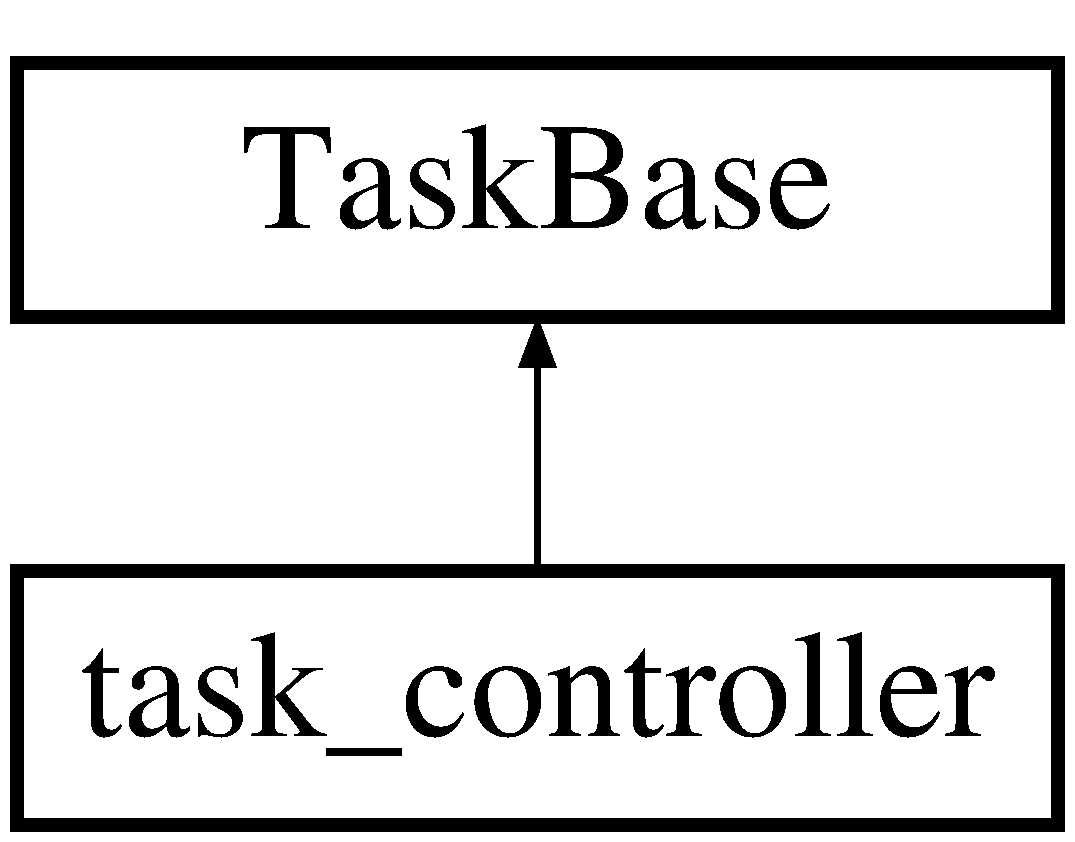
\includegraphics[height=2.000000cm]{classtask__controller}
\end{center}
\end{figure}
\subsection*{Public Member Functions}
\begin{DoxyCompactItemize}
\item 
\hyperlink{classtask__controller_a35efdd65ff9e1c4b883003ed664c0662}{task\+\_\+controller} (const char $\ast$p\+\_\+name, unsigned port\+B\+A\+S\+E\+\_\+\+T\+Y\+PE prio, size\+\_\+t stacked, emstream $\ast$serpt, \hyperlink{classBalance}{Balance} $\ast$\hyperlink{classtask__controller_a52518117258982efd9fbf567d597aa86}{controller})
\begin{DoxyCompactList}\small\item\em The constructor sets up the task object. \end{DoxyCompactList}\item 
void \hyperlink{classtask__controller_a06d4bf08d08ae59c4693028ec009bb84}{run} (void)
\begin{DoxyCompactList}\small\item\em The run method call the functions of the controller in a loop. \end{DoxyCompactList}\end{DoxyCompactItemize}
\subsection*{Protected Attributes}
\begin{DoxyCompactItemize}
\item 
\hyperlink{classBalance}{Balance} $\ast$ \hyperlink{classtask__controller_a52518117258982efd9fbf567d597aa86}{controller}\hypertarget{classtask__controller_a52518117258982efd9fbf567d597aa86}{}\label{classtask__controller_a52518117258982efd9fbf567d597aa86}

\begin{DoxyCompactList}\small\item\em The controller that is used by the task to implement the control algorithm. \end{DoxyCompactList}\end{DoxyCompactItemize}


\subsection{Detailed Description}
Task which uses accelerometer data to calculate motor actuation signals. 

This task uses the task share data made available from the I\+MU task to set the task shares for motor A and B actuation signals. 

Definition at line 28 of file task\+\_\+controller.\+h.



\subsection{Constructor \& Destructor Documentation}
\index{task\+\_\+controller@{task\+\_\+controller}!task\+\_\+controller@{task\+\_\+controller}}
\index{task\+\_\+controller@{task\+\_\+controller}!task\+\_\+controller@{task\+\_\+controller}}
\subsubsection[{\texorpdfstring{task\+\_\+controller(const char $\ast$p\+\_\+name, unsigned port\+B\+A\+S\+E\+\_\+\+T\+Y\+P\+E prio, size\+\_\+t stacked, emstream $\ast$serpt, Balance $\ast$controller)}{task_controller(const char *p_name, unsigned portBASE_TYPE prio, size_t stacked, emstream *serpt, Balance *controller)}}]{\setlength{\rightskip}{0pt plus 5cm}task\+\_\+controller\+::task\+\_\+controller (
\begin{DoxyParamCaption}
\item[{const char $\ast$}]{p\+\_\+name, }
\item[{unsigned port\+B\+A\+S\+E\+\_\+\+T\+Y\+PE}]{prio, }
\item[{size\+\_\+t}]{stacked, }
\item[{emstream $\ast$}]{serpt, }
\item[{{\bf Balance} $\ast$}]{balance\+\_\+controller}
\end{DoxyParamCaption}
)}\hypertarget{classtask__controller_a35efdd65ff9e1c4b883003ed664c0662}{}\label{classtask__controller_a35efdd65ff9e1c4b883003ed664c0662}


The constructor sets up the task object. 

Constructor for a controller object.

This constructor calls its parent class\textquotesingle{}s constructor to actually do the work of creating the controller task. 
\begin{DoxyParams}{Parameters}
{\em p\+\_\+name} & A name for this task \\
\hline
{\em prio} & The priority at which this task will run (should be low) \\
\hline
{\em stacked} & The stack space to be used by the task (not much) \\
\hline
{\em serpt} & A pointer to a serial device on which debugging messages are shown \\
\hline
{\em balance\+\_\+controller} & A pointer to a \hyperlink{classBalance}{Balance} controller used to call functions to determine the actuation signal \\
\hline
\end{DoxyParams}


Definition at line 33 of file task\+\_\+controller.\+cpp.



References controller.



\subsection{Member Function Documentation}
\index{task\+\_\+controller@{task\+\_\+controller}!run@{run}}
\index{run@{run}!task\+\_\+controller@{task\+\_\+controller}}
\subsubsection[{\texorpdfstring{run(void)}{run(void)}}]{\setlength{\rightskip}{0pt plus 5cm}void task\+\_\+controller\+::run (
\begin{DoxyParamCaption}
\item[{void}]{}
\end{DoxyParamCaption}
)}\hypertarget{classtask__controller_a06d4bf08d08ae59c4693028ec009bb84}{}\label{classtask__controller_a06d4bf08d08ae59c4693028ec009bb84}


The run method call the functions of the controller in a loop. 

The run method that calculates the actuation signal of motors x and y.

This method 

Definition at line 45 of file task\+\_\+controller.\+cpp.



References accelerometer\+\_\+\+A\+\_\+data, Balance\+::control(), controller, Balance\+::convert(), and Balance\+::set\+\_\+gains().



The documentation for this class was generated from the following files\+:\begin{DoxyCompactItemize}
\item 
\hyperlink{task__controller_8h}{task\+\_\+controller.\+h}\item 
\hyperlink{task__controller_8cpp}{task\+\_\+controller.\+cpp}\end{DoxyCompactItemize}

\hypertarget{classtask__imu}{}\section{task\+\_\+imu Class Reference}
\label{classtask__imu}\index{task\+\_\+imu@{task\+\_\+imu}}


Task which reads acceleration data from an accelerometer.  




{\ttfamily \#include $<$task\+\_\+imu.\+h$>$}

Inheritance diagram for task\+\_\+imu\+:\begin{figure}[H]
\begin{center}
\leavevmode
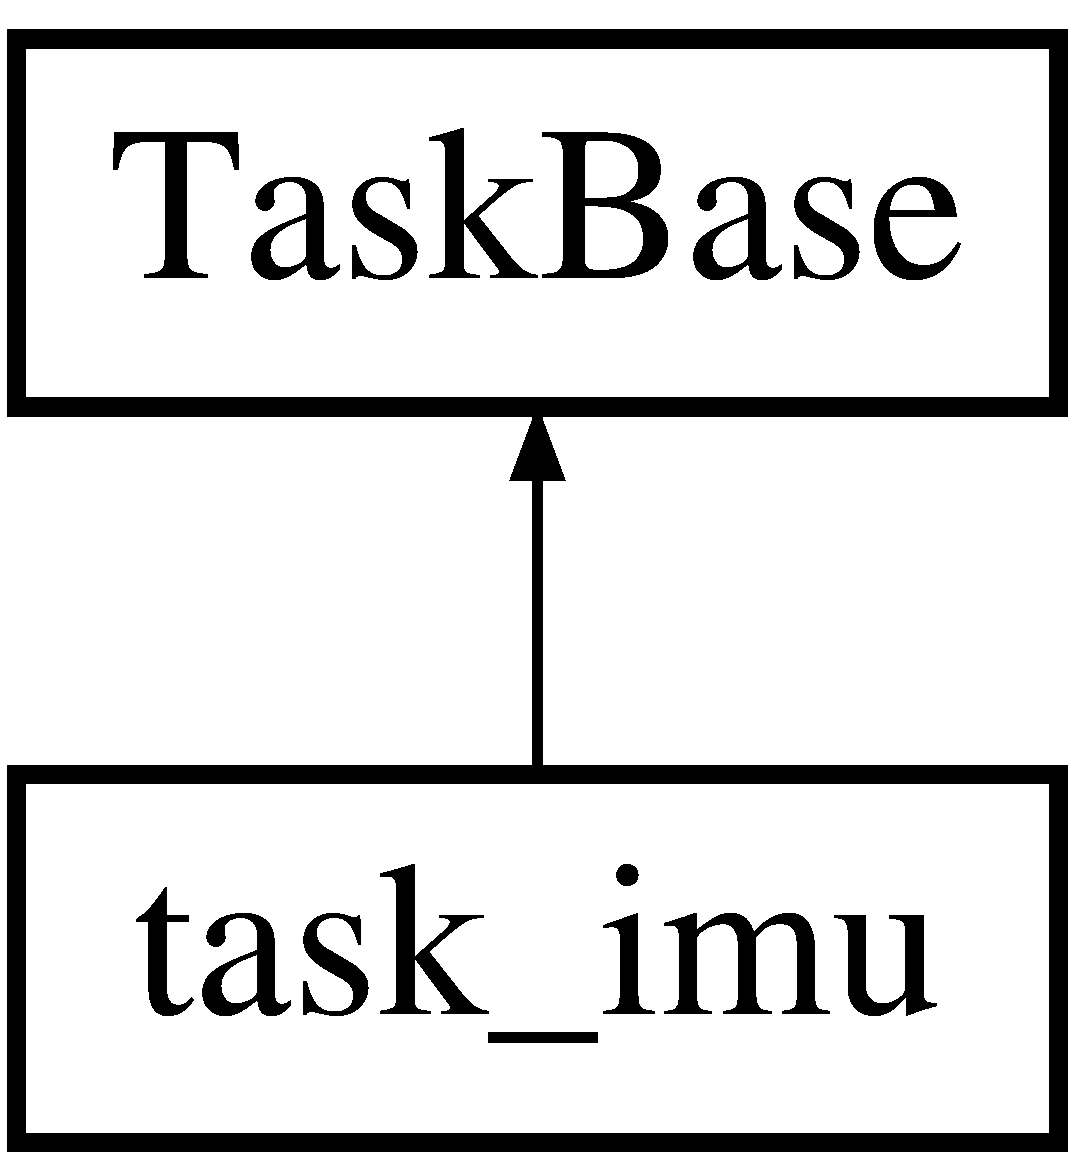
\includegraphics[height=2.000000cm]{classtask__imu}
\end{center}
\end{figure}
\subsection*{Public Member Functions}
\begin{DoxyCompactItemize}
\item 
\hyperlink{classtask__imu_a2e791d5b78ce8691e1086ea369609b74}{task\+\_\+imu} (const char $\ast$p\+\_\+name, unsigned port\+B\+A\+S\+E\+\_\+\+T\+Y\+PE prio, size\+\_\+t stacked, emstream $\ast$serpt, mma8452q $\ast$accelerometer\+In)
\begin{DoxyCompactList}\small\item\em The constructor for the task. \end{DoxyCompactList}\end{DoxyCompactItemize}
\subsection*{Protected Member Functions}
\begin{DoxyCompactItemize}
\item 
void \hyperlink{classtask__imu_ae05d282ee631de7e7c958b9a37c2651d}{run} (void)
\begin{DoxyCompactList}\small\item\em The run function for the task. No states in this run function. \end{DoxyCompactList}\end{DoxyCompactItemize}
\subsection*{Protected Attributes}
\begin{DoxyCompactItemize}
\item 
port\+Tick\+Type \hyperlink{classtask__imu_ab0a395d04d3293435477ff852ad5ebdb}{ms\+\_\+per\+\_\+sample}\hypertarget{classtask__imu_ab0a395d04d3293435477ff852ad5ebdb}{}\label{classtask__imu_ab0a395d04d3293435477ff852ad5ebdb}

\begin{DoxyCompactList}\small\item\em The number of milliseconds per sample taken by this task. \end{DoxyCompactList}\item 
mma8452q $\ast$ \hyperlink{classtask__imu_af553e9fc60df47d03c879e94487ac2fa}{accelerometer}\hypertarget{classtask__imu_af553e9fc60df47d03c879e94487ac2fa}{}\label{classtask__imu_af553e9fc60df47d03c879e94487ac2fa}

\begin{DoxyCompactList}\small\item\em A pointer to an mma8452q accelerometer used by this task. Accelerometer must be initialized and active. \end{DoxyCompactList}\item 
int16\+\_\+t \hyperlink{classtask__imu_a5b768a218bf1d4099177009f819ef8d0}{offsetA} \mbox{[}3\mbox{]} = \{-\/500, 300, 50\}\hypertarget{classtask__imu_a5b768a218bf1d4099177009f819ef8d0}{}\label{classtask__imu_a5b768a218bf1d4099177009f819ef8d0}

\begin{DoxyCompactList}\small\item\em Values used in calibration of I\+MU from its offset. \end{DoxyCompactList}\item 
float \hyperlink{classtask__imu_a255abac4e865398955b0a384c808d64b}{calibrateA} \mbox{[}3\mbox{]} = \{16.\+425, 16.\+1, 16.\+15\}\hypertarget{classtask__imu_a255abac4e865398955b0a384c808d64b}{}\label{classtask__imu_a255abac4e865398955b0a384c808d64b}

\begin{DoxyCompactList}\small\item\em Values used in calibrating I\+MU to mG. \end{DoxyCompactList}\end{DoxyCompactItemize}


\subsection{Detailed Description}
Task which reads acceleration data from an accelerometer. 

This task reads the X, Y, and Z axis accelerations from an mma8452q accelerometer and updates a task share called accelerometer\+\_\+data which is a buffer that holds the previous 5 acceleration data points 

Definition at line 25 of file task\+\_\+imu.\+h.



\subsection{Constructor \& Destructor Documentation}
\index{task\+\_\+imu@{task\+\_\+imu}!task\+\_\+imu@{task\+\_\+imu}}
\index{task\+\_\+imu@{task\+\_\+imu}!task\+\_\+imu@{task\+\_\+imu}}
\subsubsection[{\texorpdfstring{task\+\_\+imu(const char $\ast$p\+\_\+name, unsigned port\+B\+A\+S\+E\+\_\+\+T\+Y\+P\+E prio, size\+\_\+t stacked, emstream $\ast$serpt, mma8452q $\ast$accelerometer\+In)}{task_imu(const char *p_name, unsigned portBASE_TYPE prio, size_t stacked, emstream *serpt, mma8452q *accelerometerIn)}}]{\setlength{\rightskip}{0pt plus 5cm}task\+\_\+imu\+::task\+\_\+imu (
\begin{DoxyParamCaption}
\item[{const char $\ast$}]{p\+\_\+name, }
\item[{unsigned port\+B\+A\+S\+E\+\_\+\+T\+Y\+PE}]{prio, }
\item[{size\+\_\+t}]{stacked, }
\item[{emstream $\ast$}]{serpt, }
\item[{mma8452q $\ast$}]{accelerometer\+In}
\end{DoxyParamCaption}
)}\hypertarget{classtask__imu_a2e791d5b78ce8691e1086ea369609b74}{}\label{classtask__imu_a2e791d5b78ce8691e1086ea369609b74}


The constructor for the task. 

This constructor creates an imu task.


\begin{DoxyParams}{Parameters}
{\em p\+\_\+name} & A name for this task \\
\hline
{\em prio} & The priority at which this task will run \\
\hline
{\em stacked} & The stack space to be used by the task \\
\hline
{\em serpt} & A pointer to a serial device on which debugging messages are shown \\
\hline
{\em accelerometer\+In} & A pointer to an accelerometer \\
\hline
\end{DoxyParams}


Definition at line 20 of file task\+\_\+imu.\+cpp.



References accelerometer.



\subsection{Member Function Documentation}
\index{task\+\_\+imu@{task\+\_\+imu}!run@{run}}
\index{run@{run}!task\+\_\+imu@{task\+\_\+imu}}
\subsubsection[{\texorpdfstring{run(void)}{run(void)}}]{\setlength{\rightskip}{0pt plus 5cm}void task\+\_\+imu\+::run (
\begin{DoxyParamCaption}
\item[{void}]{}
\end{DoxyParamCaption}
)\hspace{0.3cm}{\ttfamily [protected]}}\hypertarget{classtask__imu_ae05d282ee631de7e7c958b9a37c2651d}{}\label{classtask__imu_ae05d282ee631de7e7c958b9a37c2651d}


The run function for the task. No states in this run function. 

The run method that runs the motor task code.

This method sets the actuation signal of each motor 

Definition at line 33 of file task\+\_\+imu.\+cpp.



References accel\+Buf\+::accel\+\_\+buffer, accelerometer, accelerometer\+\_\+\+A\+\_\+data, calibrateA, accel\+Data\+::data, and offsetA.



The documentation for this class was generated from the following files\+:\begin{DoxyCompactItemize}
\item 
\hyperlink{task__imu_8h}{task\+\_\+imu.\+h}\item 
\hyperlink{task__imu_8cpp}{task\+\_\+imu.\+cpp}\end{DoxyCompactItemize}

\hypertarget{classtask__motor}{}\section{task\+\_\+motor Class Reference}
\label{classtask__motor}\index{task\+\_\+motor@{task\+\_\+motor}}


Task which takes in an initialized motor and sets the actuation signal.  




{\ttfamily \#include $<$task\+\_\+motor.\+h$>$}

Inheritance diagram for task\+\_\+motor\+:\begin{figure}[H]
\begin{center}
\leavevmode
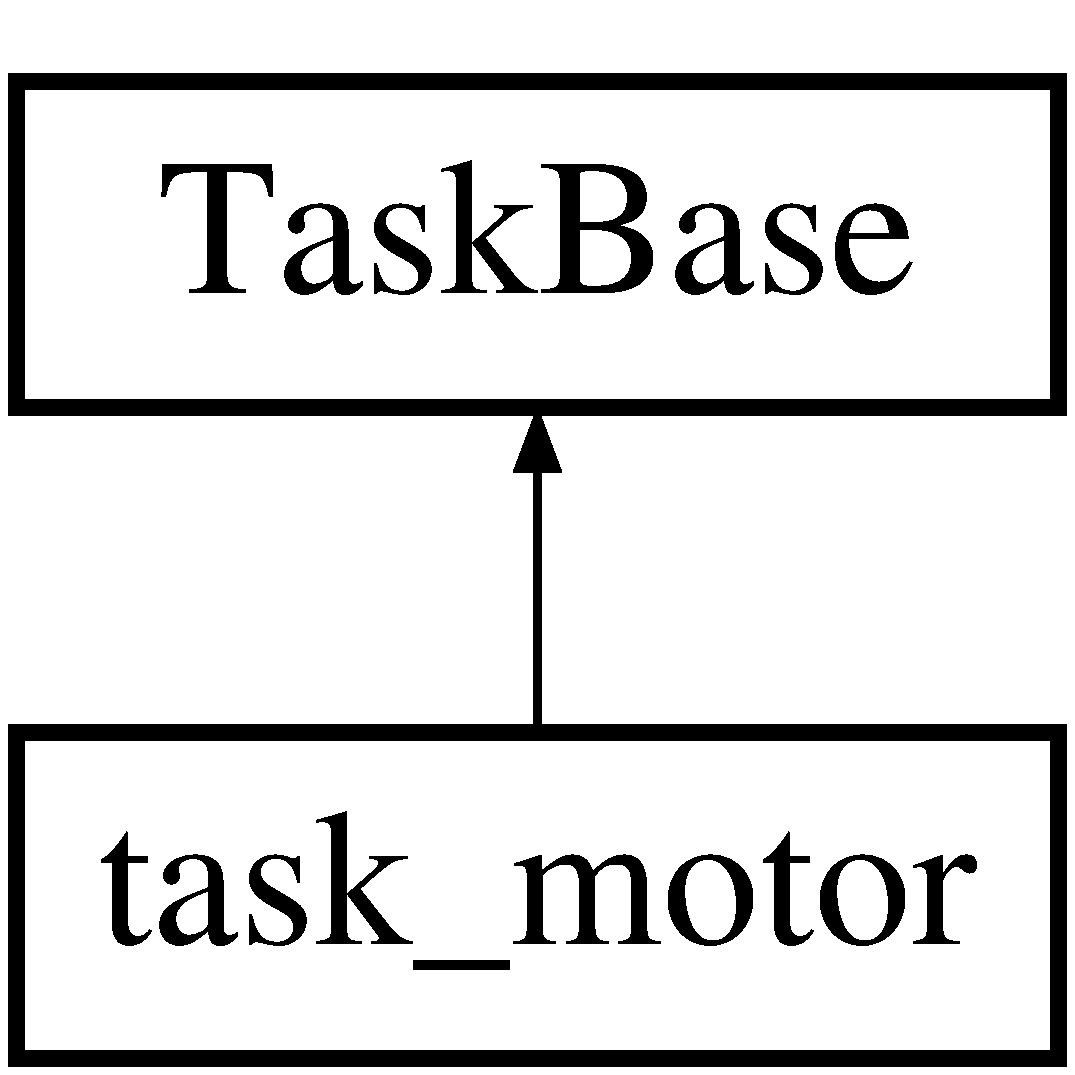
\includegraphics[height=2.000000cm]{classtask__motor}
\end{center}
\end{figure}
\subsection*{Public Member Functions}
\begin{DoxyCompactItemize}
\item 
\hyperlink{classtask__motor_a3662c77ae8591a397ba53cf1640540d8}{task\+\_\+motor} (const char $\ast$p\+\_\+name, unsigned port\+B\+A\+S\+E\+\_\+\+T\+Y\+PE prio, size\+\_\+t stacked, emstream $\ast$serpt, \hyperlink{classMotor}{Motor} $\ast$Motor\+In, uint8\+\_\+t motor\+\_\+num)
\begin{DoxyCompactList}\small\item\em This constructor creates the motor task. \end{DoxyCompactList}\end{DoxyCompactItemize}
\subsection*{Protected Member Functions}
\begin{DoxyCompactItemize}
\item 
void \hyperlink{classtask__motor_a895a075ec470c9d5a07b8959de06aacd}{run} (void)
\begin{DoxyCompactList}\small\item\em The function which does all the work for the motor task. \end{DoxyCompactList}\end{DoxyCompactItemize}
\subsection*{Protected Attributes}
\begin{DoxyCompactItemize}
\item 
port\+Tick\+Type \hyperlink{classtask__motor_a06a73825a67eaf5a5a8e31152189932f}{ms\+\_\+per\+\_\+sample}\hypertarget{classtask__motor_a06a73825a67eaf5a5a8e31152189932f}{}\label{classtask__motor_a06a73825a67eaf5a5a8e31152189932f}

\begin{DoxyCompactList}\small\item\em The number of milliseconds per sample taken by this task. \end{DoxyCompactList}\item 
\hyperlink{classMotor}{Motor} $\ast$ \hyperlink{classtask__motor_a3c6c88561488febb3bbd71aec7ba1c8f}{motor}\hypertarget{classtask__motor_a3c6c88561488febb3bbd71aec7ba1c8f}{}\label{classtask__motor_a3c6c88561488febb3bbd71aec7ba1c8f}

\begin{DoxyCompactList}\small\item\em A pointer to motor drivers used by this task. \end{DoxyCompactList}\item 
uint8\+\_\+t \hyperlink{classtask__motor_a82f00436863da33b154ce88f1735c69e}{motor\+\_\+val}\hypertarget{classtask__motor_a82f00436863da33b154ce88f1735c69e}{}\label{classtask__motor_a82f00436863da33b154ce88f1735c69e}

\begin{DoxyCompactList}\small\item\em A value to distinguish motors for the task shares used. 0 = motor\+\_\+\+A\+\_\+actuation\+Signal 1 = motor\+\_\+\+B\+\_\+actuation\+Signal. \end{DoxyCompactList}\end{DoxyCompactItemize}


\subsection{Detailed Description}
Task which takes in an initialized motor and sets the actuation signal. 

This task acquires actuation signal from a control task and sets the actuation to each motor 

Definition at line 24 of file task\+\_\+motor.\+h.



\subsection{Constructor \& Destructor Documentation}
\index{task\+\_\+motor@{task\+\_\+motor}!task\+\_\+motor@{task\+\_\+motor}}
\index{task\+\_\+motor@{task\+\_\+motor}!task\+\_\+motor@{task\+\_\+motor}}
\subsubsection[{\texorpdfstring{task\+\_\+motor(const char $\ast$p\+\_\+name, unsigned port\+B\+A\+S\+E\+\_\+\+T\+Y\+P\+E prio, size\+\_\+t stacked, emstream $\ast$serpt, Motor $\ast$\+Motor\+In, uint8\+\_\+t motor\+\_\+num)}{task_motor(const char *p_name, unsigned portBASE_TYPE prio, size_t stacked, emstream *serpt, Motor *MotorIn, uint8_t motor_num)}}]{\setlength{\rightskip}{0pt plus 5cm}task\+\_\+motor\+::task\+\_\+motor (
\begin{DoxyParamCaption}
\item[{const char $\ast$}]{p\+\_\+name, }
\item[{unsigned port\+B\+A\+S\+E\+\_\+\+T\+Y\+PE}]{prio, }
\item[{size\+\_\+t}]{stacked, }
\item[{emstream $\ast$}]{serpt, }
\item[{{\bf Motor} $\ast$}]{motor\+\_\+in, }
\item[{uint8\+\_\+t}]{motor\+\_\+num}
\end{DoxyParamCaption}
)}\hypertarget{classtask__motor_a3662c77ae8591a397ba53cf1640540d8}{}\label{classtask__motor_a3662c77ae8591a397ba53cf1640540d8}


This constructor creates the motor task. 

This constructor creates a motor task.


\begin{DoxyParams}{Parameters}
{\em p\+\_\+name} & A name for this task \\
\hline
{\em prio} & The priority at which this task will run (should be low) \\
\hline
{\em stacked} & The stack space to be used by the task (not much) \\
\hline
{\em serpt} & A pointer to a serial device on which debugging messages are shown \\
\hline
{\em motor\+\_\+in} & A pointer to a motor driver \\
\hline
{\em motor\+\_\+num} & A value to distinguish which task share to use. 0 = motorA 1 = motorB \\
\hline
\end{DoxyParams}


Definition at line 23 of file task\+\_\+motor.\+cpp.



References motor, and motor\+\_\+val.



\subsection{Member Function Documentation}
\index{task\+\_\+motor@{task\+\_\+motor}!run@{run}}
\index{run@{run}!task\+\_\+motor@{task\+\_\+motor}}
\subsubsection[{\texorpdfstring{run(void)}{run(void)}}]{\setlength{\rightskip}{0pt plus 5cm}void task\+\_\+motor\+::run (
\begin{DoxyParamCaption}
\item[{void}]{}
\end{DoxyParamCaption}
)\hspace{0.3cm}{\ttfamily [protected]}}\hypertarget{classtask__motor_a895a075ec470c9d5a07b8959de06aacd}{}\label{classtask__motor_a895a075ec470c9d5a07b8959de06aacd}


The function which does all the work for the motor task. 

The run method that runs the motor task code.

This method sets the actuation signal of the motor from the appropriate task share 

Definition at line 39 of file task\+\_\+motor.\+cpp.



References motor, motor\+\_\+\+A\+\_\+actuation\+\_\+signal, motor\+\_\+\+B\+\_\+actuation\+\_\+signal, motor\+\_\+val, and Motor\+::set\+Actuation().



The documentation for this class was generated from the following files\+:\begin{DoxyCompactItemize}
\item 
\hyperlink{task__motor_8h}{task\+\_\+motor.\+h}\item 
\hyperlink{task__motor_8cpp}{task\+\_\+motor.\+cpp}\end{DoxyCompactItemize}

\chapter{File Documentation}
\hypertarget{acceldata_8h}{}\section{acceldata.\+h File Reference}
\label{acceldata_8h}\index{acceldata.\+h@{acceldata.\+h}}


Declarations for inter-\/task data communication types.  


\subsection*{Classes}
\begin{DoxyCompactItemize}
\item 
struct \hyperlink{structaccelData}{accel\+Data}
\begin{DoxyCompactList}\small\item\em Structure to hold X, Y, and Z axis accelerations. \end{DoxyCompactList}\item 
struct \hyperlink{structaccelBuf}{accel\+Buf}
\begin{DoxyCompactList}\small\item\em Structure to hold 5 \hyperlink{structaccelData}{accel\+Data} structs. \end{DoxyCompactList}\end{DoxyCompactItemize}


\subsection{Detailed Description}
Declarations for inter-\/task data communication types. 

This file contains structs to organize data for inter-\/task communication. 
\hypertarget{Balance_8cpp}{}\section{Balance.\+cpp File Reference}
\label{Balance_8cpp}\index{Balance.\+cpp@{Balance.\+cpp}}
{\ttfamily \#include \char`\"{}Balance.\+h\char`\"{}}\\*


\subsection{Detailed Description}
This is a C++ file that implements a control loop for our ME 507 project. After hard-\/setting the PI control gains, this file should be capable of using the I\+MU sensor data to acquire an appropriate duty cycle for each motor. 
\hypertarget{main_8cpp}{}\section{main.\+cpp File Reference}
\label{main_8cpp}\index{main.\+cpp@{main.\+cpp}}


The main file for a M\+E507 balancing device.  


{\ttfamily \#include $<$math.\+h$>$}\\*
{\ttfamily \#include \char`\"{}Free\+R\+T\+O\+S.\+h\char`\"{}}\\*
{\ttfamily \#include \char`\"{}task.\+h\char`\"{}}\\*
{\ttfamily \#include \char`\"{}rs232.\+h\char`\"{}}\\*
{\ttfamily \#include \char`\"{}taskbase.\+h\char`\"{}}\\*
{\ttfamily \#include \char`\"{}taskqueue.\+h\char`\"{}}\\*
{\ttfamily \#include \char`\"{}motor\+Driver.\+h\char`\"{}}\\*
{\ttfamily \#include \char`\"{}task\+\_\+motor.\+h\char`\"{}}\\*
{\ttfamily \#include \char`\"{}task\+\_\+controller.\+h\char`\"{}}\\*
{\ttfamily \#include \char`\"{}task\+\_\+imu.\+h\char`\"{}}\\*
{\ttfamily \#include \char`\"{}Balance.\+h\char`\"{}}\\*
{\ttfamily \#include \char`\"{}acceldata.\+h\char`\"{}}\\*
\subsection*{Functions}
\begin{DoxyCompactItemize}
\item 
int \hyperlink{main_8cpp_a840291bc02cba5474a4cb46a9b9566fe}{main} (void)
\begin{DoxyCompactList}\small\item\em This function runs when the application is started up. \end{DoxyCompactList}\end{DoxyCompactItemize}
\subsection*{Variables}
\begin{DoxyCompactItemize}
\item 
Task\+Share$<$ int16\+\_\+t $>$ $\ast$ \hyperlink{main_8cpp_ae468bde2d29d8297eab6cda724eee54d}{motor\+\_\+\+A\+\_\+actuation\+\_\+signal}
\begin{DoxyCompactList}\small\item\em Pointer to a queue for text to be displayed by the UI. \end{DoxyCompactList}\item 
Task\+Share$<$ int16\+\_\+t $>$ $\ast$ \hyperlink{main_8cpp_aa376a20f7485fe6d8317ca22d7d3c8d4}{motor\+\_\+\+B\+\_\+actuation\+\_\+signal}
\begin{DoxyCompactList}\small\item\em Pointer to a share of the motor B actuation signal. \end{DoxyCompactList}\item 
Task\+Share$<$ \hyperlink{structaccelBuf}{accel\+Buf} $>$ $\ast$ \hyperlink{main_8cpp_ac12b6d4b968478cf62c26aed3a2e13aa}{accelerometer\+\_\+\+A\+\_\+data}
\begin{DoxyCompactList}\small\item\em Pointer to a share for accelerometer A data. \end{DoxyCompactList}\item 
Task\+Share$<$ \hyperlink{structaccelBuf}{accel\+Buf} $>$ $\ast$ \hyperlink{main_8cpp_a4950eab2a423bad3bf4ef929eb3c4960}{accelerometer\+\_\+\+B\+\_\+data}
\begin{DoxyCompactList}\small\item\em Pointer to a share for accelerometer B data. \end{DoxyCompactList}\end{DoxyCompactItemize}


\subsection{Detailed Description}
The main file for a M\+E507 balancing device. 

Contains the declarations to globally accessible pointers to the shared data items and queues which are used to exchange information between tasks; code which creates the pointers to the shares and queues; and the function {\ttfamily \hyperlink{main_8cpp_a840291bc02cba5474a4cb46a9b9566fe}{main()}}, which is the first function to run when the program is started up. Inside {\ttfamily \hyperlink{main_8cpp_a840291bc02cba5474a4cb46a9b9566fe}{main()}}, code does initial setup, creates the task objects which are used in the program, and starts the R\+T\+OS scheduler.

License\+: This file is copyright 2014 by JR Ridgely and released under the Lesser G\+NU Public License, version 2. It intended for educational use only, but its use is not limited thereto. 

\subsection{Function Documentation}
\index{main.\+cpp@{main.\+cpp}!main@{main}}
\index{main@{main}!main.\+cpp@{main.\+cpp}}
\subsubsection[{\texorpdfstring{main(void)}{main(void)}}]{\setlength{\rightskip}{0pt plus 5cm}int main (
\begin{DoxyParamCaption}
\item[{void}]{}
\end{DoxyParamCaption}
)}\hypertarget{main_8cpp_a840291bc02cba5474a4cb46a9b9566fe}{}\label{main_8cpp_a840291bc02cba5474a4cb46a9b9566fe}


This function runs when the application is started up. 

The {\ttfamily \hyperlink{main_8cpp_a840291bc02cba5474a4cb46a9b9566fe}{main()}} function instantiates shared variables and queues, sets up serial ports and other drivers (if needed), creates the task objects which will run {\itshape ad} {\itshape infinitum}, and starts the R\+T\+OS scheduler. \begin{DoxyReturn}{Returns}
Although the scheduler never exits and this function never returns, it\textquotesingle{}s C/\+C++ tradition for {\ttfamily \hyperlink{main_8cpp_a840291bc02cba5474a4cb46a9b9566fe}{main()}} to return an integer, so we (don\textquotesingle{}t) return zero; if the return statement is missing the compiler issues a warning. 
\end{DoxyReturn}


Definition at line 84 of file main.\+cpp.



References accelerometer\+\_\+\+A\+\_\+data, accelerometer\+\_\+\+B\+\_\+data, motor\+\_\+\+A\+\_\+actuation\+\_\+signal, and motor\+\_\+\+B\+\_\+actuation\+\_\+signal.



\subsection{Variable Documentation}
\index{main.\+cpp@{main.\+cpp}!accelerometer\+\_\+\+A\+\_\+data@{accelerometer\+\_\+\+A\+\_\+data}}
\index{accelerometer\+\_\+\+A\+\_\+data@{accelerometer\+\_\+\+A\+\_\+data}!main.\+cpp@{main.\+cpp}}
\subsubsection[{\texorpdfstring{accelerometer\+\_\+\+A\+\_\+data}{accelerometer_A_data}}]{\setlength{\rightskip}{0pt plus 5cm}Task\+Share$<${\bf accel\+Buf}$>$$\ast$ accelerometer\+\_\+\+A\+\_\+data}\hypertarget{main_8cpp_ac12b6d4b968478cf62c26aed3a2e13aa}{}\label{main_8cpp_ac12b6d4b968478cf62c26aed3a2e13aa}


Pointer to a share for accelerometer A data. 

Buffer size 10 of X,Y, and Z axis of accelerometer A 

Definition at line 66 of file main.\+cpp.



Referenced by main(), task\+\_\+controller\+::run(), and task\+\_\+imu\+::run().

\index{main.\+cpp@{main.\+cpp}!accelerometer\+\_\+\+B\+\_\+data@{accelerometer\+\_\+\+B\+\_\+data}}
\index{accelerometer\+\_\+\+B\+\_\+data@{accelerometer\+\_\+\+B\+\_\+data}!main.\+cpp@{main.\+cpp}}
\subsubsection[{\texorpdfstring{accelerometer\+\_\+\+B\+\_\+data}{accelerometer_B_data}}]{\setlength{\rightskip}{0pt plus 5cm}Task\+Share$<${\bf accel\+Buf}$>$$\ast$ accelerometer\+\_\+\+B\+\_\+data}\hypertarget{main_8cpp_a4950eab2a423bad3bf4ef929eb3c4960}{}\label{main_8cpp_a4950eab2a423bad3bf4ef929eb3c4960}


Pointer to a share for accelerometer B data. 

Buffer size 10 of X,Y, and Z axis of accelerometer B 

Definition at line 71 of file main.\+cpp.



Referenced by main().

\index{main.\+cpp@{main.\+cpp}!motor\+\_\+\+A\+\_\+actuation\+\_\+signal@{motor\+\_\+\+A\+\_\+actuation\+\_\+signal}}
\index{motor\+\_\+\+A\+\_\+actuation\+\_\+signal@{motor\+\_\+\+A\+\_\+actuation\+\_\+signal}!main.\+cpp@{main.\+cpp}}
\subsubsection[{\texorpdfstring{motor\+\_\+\+A\+\_\+actuation\+\_\+signal}{motor_A_actuation_signal}}]{\setlength{\rightskip}{0pt plus 5cm}Task\+Share$<$int16\+\_\+t$>$$\ast$ motor\+\_\+\+A\+\_\+actuation\+\_\+signal}\hypertarget{main_8cpp_ae468bde2d29d8297eab6cda724eee54d}{}\label{main_8cpp_ae468bde2d29d8297eab6cda724eee54d}


Pointer to a queue for text to be displayed by the UI. 

This queue can be used by all the tasks to print messages without having to wait for the comparatively slow serial port.\+Pointer to a share of the motor A actuation signal.

This shared pointer contains the memory address of the motorA actuation signal. 

Definition at line 55 of file main.\+cpp.



Referenced by Balance\+::control(), main(), and task\+\_\+motor\+::run().

\index{main.\+cpp@{main.\+cpp}!motor\+\_\+\+B\+\_\+actuation\+\_\+signal@{motor\+\_\+\+B\+\_\+actuation\+\_\+signal}}
\index{motor\+\_\+\+B\+\_\+actuation\+\_\+signal@{motor\+\_\+\+B\+\_\+actuation\+\_\+signal}!main.\+cpp@{main.\+cpp}}
\subsubsection[{\texorpdfstring{motor\+\_\+\+B\+\_\+actuation\+\_\+signal}{motor_B_actuation_signal}}]{\setlength{\rightskip}{0pt plus 5cm}Task\+Share$<$int16\+\_\+t$>$$\ast$ motor\+\_\+\+B\+\_\+actuation\+\_\+signal}\hypertarget{main_8cpp_aa376a20f7485fe6d8317ca22d7d3c8d4}{}\label{main_8cpp_aa376a20f7485fe6d8317ca22d7d3c8d4}


Pointer to a share of the motor B actuation signal. 

This shared pointer contains the memory address of the motorB actuation signal. 

Definition at line 61 of file main.\+cpp.



Referenced by Balance\+::control(), main(), and task\+\_\+motor\+::run().


\hypertarget{motorDriver_8cpp}{}\section{motor\+Driver.\+cpp File Reference}
\label{motorDriver_8cpp}\index{motor\+Driver.\+cpp@{motor\+Driver.\+cpp}}
{\ttfamily \#include \char`\"{}motor\+Driver.\+h\char`\"{}}\\*


\subsection{Detailed Description}
This file contains the source for a motor driver class which uses two pwm signals and an enable pin to actuate a motor. The actuation signal represents the duty cycle of the motor, which is set to be between -\/100 and 100. P\+WM is given to the motor lead pins, with only one being set at a time, and the other being set to 0\% duty cycle. 
\hypertarget{motorDriver_8h}{}\section{motor\+Driver.\+h File Reference}
\label{motorDriver_8h}\index{motor\+Driver.\+h@{motor\+Driver.\+h}}
{\ttfamily \#include \char`\"{}hw\+\_\+pwm.\+h\char`\"{}}\\*
\subsection*{Classes}
\begin{DoxyCompactItemize}
\item 
class \hyperlink{classMotor}{Motor}
\end{DoxyCompactItemize}


\subsection{Detailed Description}
This file contains a class for a motor driver which uses two pwm pins and an enable pin to control a motor. The actuation signal is saturated to between 100 and -\/100 which corresponds to a forwards and backwards 100\% duty cycle. Pwm signal is only output from one pin at a time (other pin is 0\% duty cycle) 
\hypertarget{shares_8h}{}\section{shares.\+h File Reference}
\label{shares_8h}\index{shares.\+h@{shares.\+h}}


Declarations for inter-\/task data communication items (shares and queues).  


{\ttfamily \#include \char`\"{}emstream.\+h\char`\"{}}\\*
{\ttfamily \#include \char`\"{}adc\+\_\+driver.\+h\char`\"{}}\\*
{\ttfamily \#include \char`\"{}taskshare.\+h\char`\"{}}\\*
{\ttfamily \#include \char`\"{}taskqueue.\+h\char`\"{}}\\*
{\ttfamily \#include \char`\"{}textqueue.\+h\char`\"{}}\\*
{\ttfamily \#include \char`\"{}logger\+\_\+config.\+h\char`\"{}}\\*
{\ttfamily \#include \char`\"{}acceldata.\+h\char`\"{}}\\*
\subsection*{Variables}
\begin{DoxyCompactItemize}
\item 
Task\+Share$<$ int16\+\_\+t $>$ $\ast$ \hyperlink{shares_8h_ae468bde2d29d8297eab6cda724eee54d}{motor\+\_\+\+A\+\_\+actuation\+\_\+signal}
\begin{DoxyCompactList}\small\item\em Pointer to a queue for text to be displayed by the UI. \end{DoxyCompactList}\item 
Task\+Share$<$ int16\+\_\+t $>$ $\ast$ \hyperlink{shares_8h_aa376a20f7485fe6d8317ca22d7d3c8d4}{motor\+\_\+\+B\+\_\+actuation\+\_\+signal}
\begin{DoxyCompactList}\small\item\em Pointer to a share of the motor B actuation signal. \end{DoxyCompactList}\item 
Task\+Share$<$ \hyperlink{structaccelBuf}{accel\+Buf} $>$ $\ast$ \hyperlink{shares_8h_ac12b6d4b968478cf62c26aed3a2e13aa}{accelerometer\+\_\+\+A\+\_\+data}
\begin{DoxyCompactList}\small\item\em Pointer to a share for accelerometer A data. \end{DoxyCompactList}\item 
Task\+Share$<$ \hyperlink{structaccelBuf}{accel\+Buf} $>$ $\ast$ \hyperlink{shares_8h_a4950eab2a423bad3bf4ef929eb3c4960}{accelerometer\+\_\+\+B\+\_\+data}
\begin{DoxyCompactList}\small\item\em Pointer to a share for accelerometer B data. \end{DoxyCompactList}\end{DoxyCompactItemize}


\subsection{Detailed Description}
Declarations for inter-\/task data communication items (shares and queues). 

This file contains {\ttfamily extern} declarations for queues and other inter-\/task data communication objects used in a M\+E405/507/\+Poly\+D\+AQ Free\+R\+T\+OS project.

Revisions\+: \begin{DoxyItemize}
\item 09-\/30-\/2012 J\+RR Original file was a one-\/file demonstration with two tasks \item 10-\/05-\/2012 J\+RR Split into multiple files, one for each task plus a main one \item 10-\/29-\/2012 J\+RR Reorganized with global queue and shared data references \item 06-\/18-\/2014 J\+RR Modified into Chibi\+O\+S/\+S\+T\+M32\+F4 test version\end{DoxyItemize}
License\+: This file is copyright 2014 by JR Ridgely and released under the Lesser G\+NU Public License, version 2. It intended for educational use only, but its use is not limited thereto. 

\subsection{Variable Documentation}
\index{shares.\+h@{shares.\+h}!accelerometer\+\_\+\+A\+\_\+data@{accelerometer\+\_\+\+A\+\_\+data}}
\index{accelerometer\+\_\+\+A\+\_\+data@{accelerometer\+\_\+\+A\+\_\+data}!shares.\+h@{shares.\+h}}
\subsubsection[{\texorpdfstring{accelerometer\+\_\+\+A\+\_\+data}{accelerometer_A_data}}]{\setlength{\rightskip}{0pt plus 5cm}Task\+Share$<${\bf accel\+Buf}$>$$\ast$ accelerometer\+\_\+\+A\+\_\+data}\hypertarget{shares_8h_ac12b6d4b968478cf62c26aed3a2e13aa}{}\label{shares_8h_ac12b6d4b968478cf62c26aed3a2e13aa}


Pointer to a share for accelerometer A data. 

Buffer size 10 of X,Y, and Z axis of accelerometer A 

Definition at line 66 of file main.\+cpp.



Referenced by main(), task\+\_\+controller\+::run(), and task\+\_\+imu\+::run().

\index{shares.\+h@{shares.\+h}!accelerometer\+\_\+\+B\+\_\+data@{accelerometer\+\_\+\+B\+\_\+data}}
\index{accelerometer\+\_\+\+B\+\_\+data@{accelerometer\+\_\+\+B\+\_\+data}!shares.\+h@{shares.\+h}}
\subsubsection[{\texorpdfstring{accelerometer\+\_\+\+B\+\_\+data}{accelerometer_B_data}}]{\setlength{\rightskip}{0pt plus 5cm}Task\+Share$<${\bf accel\+Buf}$>$$\ast$ accelerometer\+\_\+\+B\+\_\+data}\hypertarget{shares_8h_a4950eab2a423bad3bf4ef929eb3c4960}{}\label{shares_8h_a4950eab2a423bad3bf4ef929eb3c4960}


Pointer to a share for accelerometer B data. 

Buffer size 10 of X,Y, and Z axis of accelerometer B 

Definition at line 71 of file main.\+cpp.



Referenced by main().

\index{shares.\+h@{shares.\+h}!motor\+\_\+\+A\+\_\+actuation\+\_\+signal@{motor\+\_\+\+A\+\_\+actuation\+\_\+signal}}
\index{motor\+\_\+\+A\+\_\+actuation\+\_\+signal@{motor\+\_\+\+A\+\_\+actuation\+\_\+signal}!shares.\+h@{shares.\+h}}
\subsubsection[{\texorpdfstring{motor\+\_\+\+A\+\_\+actuation\+\_\+signal}{motor_A_actuation_signal}}]{\setlength{\rightskip}{0pt plus 5cm}Task\+Share$<$int16\+\_\+t$>$$\ast$ motor\+\_\+\+A\+\_\+actuation\+\_\+signal}\hypertarget{shares_8h_ae468bde2d29d8297eab6cda724eee54d}{}\label{shares_8h_ae468bde2d29d8297eab6cda724eee54d}


Pointer to a queue for text to be displayed by the UI. 

This queue can be used by all the tasks to print messages without having to wait for the comparatively slow serial port.\+Pointer to a share of the motor A actuation signal.

This shared pointer contains the memory address of the motorA actuation signal. 

Definition at line 55 of file main.\+cpp.



Referenced by Balance\+::control(), main(), and task\+\_\+motor\+::run().

\index{shares.\+h@{shares.\+h}!motor\+\_\+\+B\+\_\+actuation\+\_\+signal@{motor\+\_\+\+B\+\_\+actuation\+\_\+signal}}
\index{motor\+\_\+\+B\+\_\+actuation\+\_\+signal@{motor\+\_\+\+B\+\_\+actuation\+\_\+signal}!shares.\+h@{shares.\+h}}
\subsubsection[{\texorpdfstring{motor\+\_\+\+B\+\_\+actuation\+\_\+signal}{motor_B_actuation_signal}}]{\setlength{\rightskip}{0pt plus 5cm}Task\+Share$<$int16\+\_\+t$>$$\ast$ motor\+\_\+\+B\+\_\+actuation\+\_\+signal}\hypertarget{shares_8h_aa376a20f7485fe6d8317ca22d7d3c8d4}{}\label{shares_8h_aa376a20f7485fe6d8317ca22d7d3c8d4}


Pointer to a share of the motor B actuation signal. 

This shared pointer contains the memory address of the motorB actuation signal. 

Definition at line 61 of file main.\+cpp.



Referenced by Balance\+::control(), main(), and task\+\_\+motor\+::run().


\hypertarget{task__controller_8cpp}{}\section{task\+\_\+controller.\+cpp File Reference}
\label{task__controller_8cpp}\index{task\+\_\+controller.\+cpp@{task\+\_\+controller.\+cpp}}
{\ttfamily \#include \char`\"{}task\+\_\+controller.\+h\char`\"{}}\\*


\subsection{Detailed Description}
This file contains source code for a motor controller. This task serves to output the appropriate duty cycle corresponding to the effort of the motor necessary to correct the position of the platform.

Revisions\+: \begin{DoxyItemize}
\item 11-\/29-\/2018 L\+EW Original file\end{DoxyItemize}
Accreditation\+: The structure of this file, organization and some content, was directly written by John Ridgely, 11-\/26-\/2012. I have been given his files and explicit permission to adapt said files for ME 507 project use. 
\hypertarget{task__controller_8h}{}\section{task\+\_\+controller.\+h File Reference}
\label{task__controller_8h}\index{task\+\_\+controller.\+h@{task\+\_\+controller.\+h}}
{\ttfamily \#include \char`\"{}Free\+R\+T\+O\+S.\+h\char`\"{}}\\*
{\ttfamily \#include \char`\"{}task.\+h\char`\"{}}\\*
{\ttfamily \#include \char`\"{}Balance.\+h\char`\"{}}\\*
{\ttfamily \#include \char`\"{}taskbase.\+h\char`\"{}}\\*
{\ttfamily \#include \char`\"{}shares.\+h\char`\"{}}\\*
\subsection*{Classes}
\begin{DoxyCompactItemize}
\item 
class \hyperlink{classtask__controller}{task\+\_\+controller}
\begin{DoxyCompactList}\small\item\em Task which uses accelerometer data to calculate motor actuation signals. \end{DoxyCompactList}\end{DoxyCompactItemize}


\subsection{Detailed Description}
This file contains headers for a motor controller. This task serves to output the appropriate duty cycle corresponding to the effort of the motor necessary to correct the position of the platform. 
\hypertarget{task__imu_8cpp}{}\section{task\+\_\+imu.\+cpp File Reference}
\label{task__imu_8cpp}\index{task\+\_\+imu.\+cpp@{task\+\_\+imu.\+cpp}}
{\ttfamily \#include \char`\"{}task\+\_\+imu.\+h\char`\"{}}\\*


\subsection{Detailed Description}
This file contains the source for an imu task which initializes two mma8451\textquotesingle{}s and save there data to a share 
\hypertarget{task__imu_8h}{}\section{task\+\_\+imu.\+h File Reference}
\label{task__imu_8h}\index{task\+\_\+imu.\+h@{task\+\_\+imu.\+h}}
{\ttfamily \#include \char`\"{}taskbase.\+h\char`\"{}}\\*
{\ttfamily \#include \char`\"{}shares.\+h\char`\"{}}\\*
{\ttfamily \#include \char`\"{}mma8452q.\+h\char`\"{}}\\*
{\ttfamily \#include \char`\"{}emstream.\+h\char`\"{}}\\*
\subsection*{Classes}
\begin{DoxyCompactItemize}
\item 
class \hyperlink{classtask__imu}{task\+\_\+imu}
\begin{DoxyCompactList}\small\item\em Task which reads acceleration data from an accelerometer. \end{DoxyCompactList}\end{DoxyCompactItemize}


\subsection{Detailed Description}
This file contains the headers for an imu task which initializes two mma8451\textquotesingle{}s and sets there actuation signal when run is called. 
\hypertarget{task__motor_8cpp}{}\section{task\+\_\+motor.\+cpp File Reference}
\label{task__motor_8cpp}\index{task\+\_\+motor.\+cpp@{task\+\_\+motor.\+cpp}}
{\ttfamily \#include \char`\"{}emstream.\+h\char`\"{}}\\*
{\ttfamily \#include \char`\"{}task\+\_\+motor.\+h\char`\"{}}\\*


\subsection{Detailed Description}
This file contains the source for a motor task which is a child of basetask. It takes an initialized motor driver and a motor value and sets the actuatuon of the motor using a task share. The motor value distinguishes which task share to use. 
\hypertarget{task__motor_8h}{}\section{task\+\_\+motor.\+h File Reference}
\label{task__motor_8h}\index{task\+\_\+motor.\+h@{task\+\_\+motor.\+h}}
{\ttfamily \#include \char`\"{}taskbase.\+h\char`\"{}}\\*
{\ttfamily \#include \char`\"{}shares.\+h\char`\"{}}\\*
{\ttfamily \#include \char`\"{}motor\+Driver.\+h\char`\"{}}\\*
\subsection*{Classes}
\begin{DoxyCompactItemize}
\item 
class \hyperlink{classtask__motor}{task\+\_\+motor}
\begin{DoxyCompactList}\small\item\em Task which takes in an initialized motor and sets the actuation signal. \end{DoxyCompactList}\end{DoxyCompactItemize}


\subsection{Detailed Description}
This file contains the headers for a motor task which takes a motor\+Driver object and sets its actuation signal according to a task share 
%--- End generated contents ---

% Index
\backmatter
\newpage
\phantomsection
\clearemptydoublepage
\addcontentsline{toc}{chapter}{Index}
\printindex

\end{document}
